\section{The Bernoulli Hash Function family}
\label{sec:shf}

The \emph{Bernoulli Hash Function} (BHF) is a family of constructions that
encode a finite set or map into a compact binary representation using a hash
function and a \emph{salt}---a bit string $b$ discovered by search.
The key idea is an \emph{acceptance predicate} that determines membership.

\subsection{Acceptance predicates}

\begin{definition}[Acceptance predicate]
\label{def:acceptance}
Given a hash function $\hash$, a salt $b \in \cisb$, a modulus $N \in \NatSet$,
and an \emph{acceptance set} $\Set{A} \subseteq \{0, 1, \ldots, N-1\}$, an
element $x$ is \emph{accepted} if and only if
\begin{equation}
    \hash(x \cat b) \bmod N \in \Set{A}\,.
\end{equation}
Under the random oracle assumption (\cref{asm:ro_approx}), the false positive
rate is
\begin{equation}
    \fprate = \frac{\Card{\Set{A}}}{N}\,.
\end{equation}
\end{definition}

Two important special cases arise from the choice of $\Set{A}$:

\paragraph{Equality predicate (classical BHF).}
Set $N = 2^k$ and $\Set{A} = \{h_0\}$ for some $h_0 \in \{0,\ldots,2^k-1\}$
discovered adaptively during construction.
Then $\fprate = 2^{-k}$ and the membership test is
\begin{equation}
    \hash(x \cat b) \bmod 2^k = h_0\,.
\end{equation}
The achievable false positive rates are $\fprate \in \{2^{-k} : k \in \NatSet\}$.

\paragraph{Threshold predicate (generalization).}
Set $\Set{A} = \{0, 1, \ldots, t\}$ for a threshold $t \geq 0$.
Then $\fprate = (t+1)/N$ and the membership test is
\begin{equation}
\label{eq:threshold_test}
    \hash(x \cat b) \bmod N \leq t\,.
\end{equation}
The achievable false positive rates are
$\fprate \in \{j/N : j = 1, \ldots, N\}$, which is a much finer lattice
than the power-of-two constraint of the equality predicate.

\subsection{Success probability per trial}

The probability that a candidate salt $b$ produces a valid BHF depends on the
predicate type.

\begin{theorem}[Success probability---equality predicate]
\label{thm:success_eq}
For the equality predicate with $m$ keys, false positive rate
$\fprate = 2^{-k}$, and mean value encoding length $\mu$ bits, the probability
that a given salt $b$ yields a valid construction is
\begin{equation}
    p_{\mathrm{eq}}(m, \fprate, \mu) = \frac{\fprate^{m-1}}{2^{m\mu}}\,.
\end{equation}
\end{theorem}
\begin{proof}
Under the random oracle assumption, the hash of each key concatenated with
$b$ is independent and uniform.
The first key fixes the target hash $h_0$; each of the remaining $m-1$ keys
must hash to $h_0$, each with probability $\fprate$.
Additionally, for a map, each key's value must match the first $\BL(v_i)$ bits
of a second hash, contributing a factor of $2^{-\BL(v_i)}$ per key.
The product is
\begin{equation}
    \fprate^{m-1} \cdot \prod_{i=1}^{m} 2^{-\BL(v_i)}
    = \frac{\fprate^{m-1}}{2^{m\mu}}\,,
\end{equation}
where $\mu = \frac{1}{m}\sum_{i=1}^{m} \BL(v_i)$ is the mean value bit length.
For sets, $\mu = 0$ and the expression reduces to $\fprate^{m-1}$.
\end{proof}

\begin{theorem}[Success probability---threshold predicate]
\label{thm:success_thresh}
For the threshold predicate with modulus $N$, threshold $t$, $m$ keys, and mean
value encoding length $\mu$ bits, the probability that a given salt $b$ yields
a valid construction is
\begin{equation}
    p_{\mathrm{th}}(m, \fprate, \mu) = \frac{\fprate^{m}}{2^{m\mu}}\,.
\end{equation}
\end{theorem}
\begin{proof}
With the threshold predicate, the acceptance set $\Set{A} = \{0,\ldots,t\}$ is
fixed \emph{before} examining the salt.
Each of the $m$ keys must independently hash into $\Set{A}$, each with
probability $\fprate = (t+1)/N$.
This gives $\fprate^m$ (not $\fprate^{m-1}$, since no key is ``free'' to fix
the target).
The value-matching factor contributes $2^{-m\mu}$ as before.
\end{proof}

\begin{remark}
The equality predicate has a factor-of-$\fprate^{-1}$ advantage in success
probability because one key adaptively determines $h_0$.
In the space complexity (\cref{sec:space}), this manifests as an additive
$\log_2 \fprate / m$ bits per element, which vanishes as $m \to \infty$.
Both predicates achieve the same asymptotic optimum.
\end{remark}

\subsection{FPR granularity}

\begin{theorem}[FPR granularity]
\label{thm:fpr_granularity}
With modulus $N$, the threshold predicate achieves any false positive rate in
the lattice
\begin{equation}
    \fprate \in \left\{\frac{j}{N} : j = 1, 2, \ldots, N\right\}\,,
\end{equation}
whereas the equality predicate achieves only
$\fprate \in \{2^{-k} : k \in \NatSet\}$.
\end{theorem}

This is immediate from the definitions.
For example, with $N = 100$, one can achieve $\fprate = 0.01, 0.02, \ldots, 1.00$, whereas the equality predicate can only achieve $\fprate = 0.5, 0.25, 0.125, \ldots$

\subsection{Simplified search for $\fnrate > 0$}

When the false negative rate $\fnrate > 0$, only $p = (1-\fnrate)m$ of the
$m$ elements need to be accepted.
Under the equality predicate, the algorithm must enumerate all $\binom{m}{p}$
subsets of size $p$ and check whether each subset collides.
Under the threshold predicate, the search is dramatically simpler.

\begin{theorem}[Search complexity for $\fnrate > 0$]
\label{thm:fnr_search}
Under the threshold predicate, testing whether a candidate salt $b$ admits at
least $p$ of $m$ elements requires $\mathcal{O}(m)$ hash evaluations: simply
count how many elements satisfy $\hash(x \cat b) \bmod N \leq t$.

Under the equality predicate, the same test requires
$\mathcal{O}\!\left(\binom{m}{p} \cdot m\right)$ hash evaluations in the worst
case, since each candidate $h_0$ (determined by each $p$-subset) must be
checked against all elements.
\end{theorem}
\begin{proof}
For the threshold predicate, the acceptance set $\Set{A}$ is fixed.
For each candidate salt $b$, we compute $\hash(x_i \cat b) \bmod N$ for
$i = 1,\ldots,m$ and count the number that fall in $\Set{A}$.
If at least $p$ do, the salt succeeds.
This is $\mathcal{O}(m)$ per candidate salt.

For the equality predicate, the target $h_0$ is not known a priori.
For each $p$-element subset, the first element determines $h_0$, and the
remaining $p-1$ elements must match.
Since there are $\binom{m}{p}$ such subsets, the worst-case cost per candidate
salt is $\mathcal{O}\!\left(\binom{m}{p} \cdot m\right)$.
\end{proof}

\subsection{Adaptive threshold}
\label{sec:adaptive}

The equality and threshold predicates both fix the acceptance set \emph{before}
examining the data, then search for a salt that maps all (or enough) elements
into it.
An alternative is to let the data \emph{determine} the threshold.

\begin{definition}[Adaptive threshold predicate]
\label{def:adaptive_threshold}
Given a salt $b \in \cisb$, a modulus $N$, and $m$ keys
$x_1,\ldots,x_m$, compute the residues
\begin{equation}
    r_i \;=\; \hash(x_i \cat b) \bmod N\,, \quad i = 1,\ldots,m\,,
\end{equation}
and let $\OS{p}{m}$ denote the $p$-th order statistic (the $p$-th smallest
value among $r_1,\ldots,r_m$).
Set the threshold $t = \OS{p}{m}$.
An element $x$ is accepted if and only if
\begin{equation}
\label{eq:adaptive_test}
    \hash(x \cat b) \bmod N \leq t\,.
\end{equation}
By construction, at least $p$ of the $m$ keys are accepted.
The false positive rate is the random variable
\begin{equation}
\label{eq:adaptive_fpr}
    \fprate \;=\; \frac{\OS{p}{m} + 1}{N}\,.
\end{equation}
\end{definition}

\begin{remark}
Unlike the fixed-threshold predicate, the adaptive threshold produces a
\emph{random} false positive rate that depends on the particular salt and keys.
The parameter $p$ controls the expected FPR: choosing
$p = \lfloor \epsilon^{*}(m+1) \rfloor$ targets a desired mean FPR of
$\epsilon^{*}$.
\end{remark}

\subsubsection{Success probability}

\begin{theorem}[Success probability---adaptive threshold, sets]
\label{thm:success_adaptive_set}
For the adaptive threshold predicate applied to a Bernoulli set ($\mu = 0$)
with $m$ keys and $p \leq m$, every candidate salt $b$ yields a valid
construction.
The success probability per trial is
\begin{equation}
    p_{\mathrm{ad}} = 1\,.
\end{equation}
\end{theorem}
\begin{proof}
For any salt $b$, the $m$ residues $r_1,\ldots,r_m$ are well-defined.
We sort them and set $t = \OS{p}{m}$.
By the definition of the $p$-th order statistic, at least $p$ residues
satisfy $r_i \leq t$.
Since there is no value-matching constraint ($\mu = 0$), every salt succeeds.
No search is required.
\end{proof}

\begin{theorem}[Success probability---adaptive threshold, maps]
\label{thm:success_adaptive_map}
For the adaptive threshold predicate applied to a Bernoulli map ($\mu > 0$)
with $m$ keys and value encoding lengths $\BL(v_1),\ldots,\BL(v_m)$, the
success probability per trial is
\begin{equation}
\label{eq:success_adaptive_map}
    p_{\mathrm{ad}}(m, p, \mu)
    \;=\; \Prob{\Card{\Set{V}} \geq p}\,,
\end{equation}
where $\Set{V} = \{i : \hash(1 \cat x_i \cat b) \bmod 2^{\BL(v_i)} =
\Encode(v_i)\}$ is the set of value-matching keys and
$\Card{\Set{V}} \sim \bindist(m, 2^{-\mu})$ under the random oracle
assumption.
\end{theorem}
\begin{proof}
The value-matching constraint is independent of the residue ordering.
For each key $x_i$, the value hash matches with probability $2^{-\BL(v_i)}$.
Under the random oracle assumption, these are independent Bernoulli trials, so
$\Card{\Set{V}} \sim \bindist(m, 2^{-\mu})$ (exactly when all values have the
same encoding length; approximately otherwise).
The adaptive threshold can be set on any $p$ of the value-matching keys, so the
salt succeeds if and only if $\Card{\Set{V}} \geq p$.
\end{proof}

\begin{corollary}
\label{cor:adaptive_no_search}
For Bernoulli sets, the adaptive threshold eliminates the salt search entirely:
the first (and only) candidate salt $b$ always succeeds.
The construction time is $\mathcal{O}(m \log m)$ (dominated by sorting the
residues).
\end{corollary}

\subsubsection{FPR distribution}

Under the random oracle assumption, the residues $r_1,\ldots,r_m$ are i.i.d.\
uniform on $\{0,1,\ldots,N-1\}$.
The threshold $t = \OS{p}{m}$ is therefore the $p$-th order statistic of $m$
i.i.d.\ discrete uniform random variables.

\begin{theorem}[Exact FPR distribution]
\label{thm:fpr_distribution}
For sets ($\mu = 0$), the threshold $T = \OS{p}{m}$ has the probability mass
function
\begin{equation}
\label{eq:os_pmf}
    \Prob{T = j}
    \;=\; \frac{\binom{j}{p-1}\binom{N-1-j}{m-p}}{\binom{N-1}{m-1}}
    \cdot \frac{m}{N}\,,
    \quad j = p-1, p, \ldots, N-1-(m-p)\,,
\end{equation}
which is the PMF of the $p$-th order statistic from $m$ i.i.d.\
$\operatorname{Uniform}\{0,\ldots,N-1\}$ draws.
Equivalently, $T + 1$ follows a
$\operatorname{BetaBinomial}(N, p, m - p + 1)$ distribution shifted by $p$.

In the continuous limit ($N \to \infty$ with $\fprate = (T+1)/N$), the FPR
converges in distribution:
\begin{equation}
\label{eq:fpr_beta}
    \fprate \;\xrightarrow{d}\; \betadist(p,\; m - p + 1)\,.
\end{equation}
\end{theorem}
\begin{proof}
See \cref{sec:adaptive_pmf_derivation} for the exact discrete derivation.
The continuous limit follows from the classical result that the $p$-th order
statistic of $m$ i.i.d.\ $\operatorname{Uniform}(0,1)$ random variables has
a $\betadist(p, m - p + 1)$
distribution~\cite{order_statistics}.
\end{proof}

\begin{theorem}[Moments of the adaptive FPR]
\label{thm:adaptive_moments}
In the continuous limit, the expected FPR and its variance are
\begin{align}
\label{eq:adaptive_mean}
    \Expect{\fprate} &= \frac{p}{m + 1}\,, \\
\label{eq:adaptive_var}
    \Var{\fprate} &= \frac{p(m - p + 1)}{(m + 1)^2(m + 2)}\,.
\end{align}
To target a desired mean FPR of $\epsilon^{*}$, choose
\begin{equation}
\label{eq:adaptive_p_choice}
    p = \lfloor \epsilon^{*}(m + 1) \rfloor\,.
\end{equation}
The variance $\Var{\fprate} = \mathcal{O}(1/m)$ vanishes as $m \to \infty$,
so the FPR concentrates around $\epsilon^{*}$.
\end{theorem}
\begin{proof}
These are the moments of the $\betadist(p, m - p + 1)$ distribution:
$\Expect{X} = \alpha / (\alpha + \beta)$ and
$\Var{X} = \alpha\beta / ((\alpha + \beta)^2(\alpha + \beta + 1))$
with $\alpha = p$ and $\beta = m - p + 1$.
\end{proof}

\begin{remark}
For maps ($\mu > 0$), the FPR distribution is a mixture: conditioned on the
number of value-matching keys $\Card{\Set{V}} = v \geq p$, the threshold is the
$p$-th order statistic of $v$ residues.
The unconditional FPR is
\begin{equation}
    \fprate \mid \Card{\Set{V}} = v \;\sim\; \betadist(p, v - p + 1)\,,
\end{equation}
and the marginal FPR averages over $\Card{\Set{V}} \sim \bindist(m, 2^{-\mu})$
restricted to $\Card{\Set{V}} \geq p$.
\end{remark}

\subsubsection{Search complexity}

\begin{theorem}[Construction complexity---adaptive threshold]
\label{thm:adaptive_complexity}
The construction time for the adaptive threshold predicate is:
\begin{enumerate}[(i)]
    \item Sets ($\mu = 0$): $\mathcal{O}(m \log m)$ (one pass, dominated by
    sorting the $m$ residues).
    \item Maps ($\mu > 0$): Expected $\mathcal{O}(m \log m / p_{\mathrm{ad}})$,
    where $p_{\mathrm{ad}} = \Prob{\Card{\Set{V}} \geq p}$.
    Each trial costs $\mathcal{O}(m \log m)$ and the expected number of trials
    is $1 / p_{\mathrm{ad}}$.
\end{enumerate}
\end{theorem}
\begin{proof}
For sets, the construction hashes $m$ elements ($\mathcal{O}(m)$), sorts the
residues ($\mathcal{O}(m \log m)$), and reads off $t = \OS{p}{m}$.
No search is needed (\cref{thm:success_adaptive_set}).

For maps, each candidate salt requires $\mathcal{O}(m)$ hash evaluations to
identify value-matching keys and $\mathcal{O}(m \log m)$ to sort residues.
The geometric search terminates after an expected $1/p_{\mathrm{ad}}$ trials.
\end{proof}

\subsubsection{Comparison of predicates}

\begin{table}[ht]
\centering
\caption{Comparison of the three acceptance predicates for the BHF.}
\label{tab:predicate_comparison}
\begin{tabular}{lccc}
\hline
 & \textbf{Equality} & \textbf{Threshold} & \textbf{Adaptive} \\
\hline
FPR type & fixed & fixed & random \\
FPR values ($\mu=0$) & $\{2^{-k}\}$ & $\{j/N\}$ & $\betadist(p,m\!-\!p\!+\!1)$ \\
Success prob.\ (sets) & $\fprate^{m-1}$ & $\fprate^{m}$ & $1$ \\
Salt search & geometric & geometric & none (sets) \\
Construction & $\mathcal{O}(m/p)$ trials & $\mathcal{O}(m/p)$ trials & $\mathcal{O}(m \log m)$ \\
Stored params & $(h_k, b)$ & $(N, t, b)$ & $(N, t)$ \\
Bits/element & $-\!\log_2\!\fprate + \mu$ & $-\!\log_2\!\fprate + \mu$ & $\mathcal{O}(\log N / m)$ \\
Max entropy? & yes & yes & no (see \cref{sec:adaptive_entropy}) \\
\hline
\end{tabular}
\end{table}

\subsubsection{Adaptive FPR distribution}

\Cref{fig:adaptive_fpr} shows the $\betadist(p, m - p + 1)$ density for
several choices of $(m, p)$.
As $m$ grows, the density concentrates around the mean $p/(m+1)$.

\begin{figure}[ht]
\centering
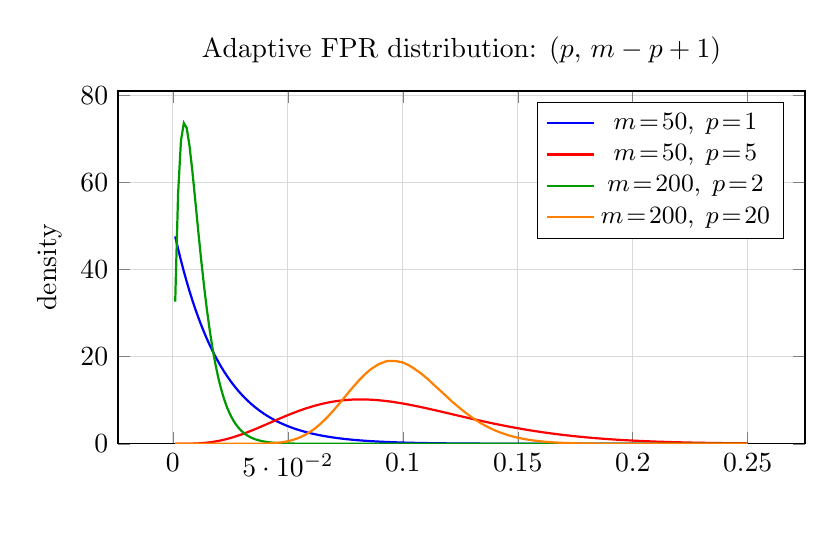
\begin{tikzpicture}
\begin{axis}[
    width=0.85\textwidth,
    height=0.5\textwidth,
    xlabel={$\fprate$},
    ylabel={density},
    domain=0.001:0.25,
    samples=200,
    legend style={at={(0.97,0.97)}, anchor=north east, font=\small},
    ymin=0,
    grid=major,
    grid style={gray!30},
    every axis plot/.append style={thick, no markers},
    title={Adaptive FPR distribution: $\betadist(p,\, m - p + 1)$}
]
% Beta PDF: f(x) = x^(a-1)(1-x)^(b-1) / B(a,b)
% We use pgfplots math; gamma function via ln(x!) trick not available,
% so we normalise visually using the known mode and scale.

% (m=50, p=1): Beta(1,50) -- exponential-like
\addplot[blue] {(1-x)^49 * 50};
\addlegendentry{$m\!=\!50,\; p\!=\!1$}

% (m=50, p=5): Beta(5,46)
\addplot[red] {x^4 * (1-x)^45 * 50! / (4! * 45!)};
\addlegendentry{$m\!=\!50,\; p\!=\!5$}

% (m=200, p=2): Beta(2,199)
\addplot[green!60!black] {x * (1-x)^198 * 200*199};
\addlegendentry{$m\!=\!200,\; p\!=\!2$}

% (m=200, p=20): Beta(20,181)
\addplot[orange] {
    exp(
        19*ln(x) + 180*ln(1-x)
        + ln(200!) - ln(19!) - ln(180!)
    )
};
\addlegendentry{$m\!=\!200,\; p\!=\!20$}

\end{axis}
\end{tikzpicture}
\caption{The $\betadist(p, m-p+1)$ density of the adaptive FPR for several
    $(m,p)$ pairs.
    As $m$ grows (green, orange curves), the density concentrates around the
    mean $\Expect{\fprate} = p/(m+1)$.
    For $p = 1$ (blue), the density is a decaying exponential concentrated near
    zero.}
\label{fig:adaptive_fpr}
\end{figure}
